\vspace{2mm}
\tikzset{every picture/.style={line width=0.75pt}} %set default line width to 0.75pt        

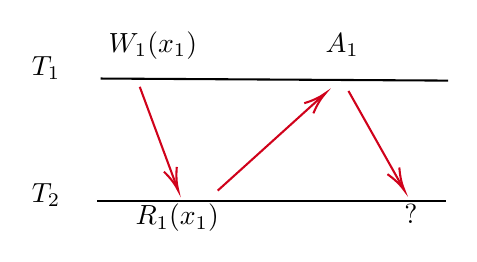
\begin{tikzpicture}[x=0.75pt,y=0.75pt,yscale=-1,xscale=1]
%uncomment if require: \path (0,300); %set diagram left start at 0, and has height of 300

%Straight Lines [id:da9500410641573396] 
\draw    (49.17,42) -- (216.56,43) ;
%Straight Lines [id:da7796185686481738] 
\draw    (47.56,101) -- (215.76,101) ;
%Straight Lines [id:da9563274467788809] 
\draw [color={rgb, 255:red, 208; green, 2; blue, 27 }  ,draw opacity=1 ]   (68,46) -- (85.86,94.13) ;
\draw [shift={(86.56,96)}, rotate = 249.64] [color={rgb, 255:red, 208; green, 2; blue, 27 }  ,draw opacity=1 ][line width=0.75]    (10.93,-3.29) .. controls (6.95,-1.4) and (3.31,-0.3) .. (0,0) .. controls (3.31,0.3) and (6.95,1.4) .. (10.93,3.29)   ;
%Straight Lines [id:da9159237520413861] 
\draw [color={rgb, 255:red, 208; green, 2; blue, 27 }  ,draw opacity=1 ]   (105.56,96) -- (156.08,50.34) ;
\draw [shift={(157.56,49)}, rotate = 137.89] [color={rgb, 255:red, 208; green, 2; blue, 27 }  ,draw opacity=1 ][line width=0.75]    (10.93,-3.29) .. controls (6.95,-1.4) and (3.31,-0.3) .. (0,0) .. controls (3.31,0.3) and (6.95,1.4) .. (10.93,3.29)   ;
%Straight Lines [id:da9009499956012581] 
\draw [color={rgb, 255:red, 208; green, 2; blue, 27 }  ,draw opacity=1 ]   (168.56,48) -- (194.58,94.26) ;
\draw [shift={(195.56,96)}, rotate = 240.64] [color={rgb, 255:red, 208; green, 2; blue, 27 }  ,draw opacity=1 ][line width=0.75]    (10.93,-3.29) .. controls (6.95,-1.4) and (3.31,-0.3) .. (0,0) .. controls (3.31,0.3) and (6.95,1.4) .. (10.93,3.29)   ;

% Text Node
\draw (14.5,30) node [anchor=north west][inner sep=0.75pt]   [align=left] {$T_1$};
% Text Node
\draw (51.56,18) node [anchor=north west][inner sep=0.75pt]   [align=left] {$W_1(x_1)$};
% Text Node
\draw (156,19) node [anchor=north west][inner sep=0.75pt]   [align=left] {$A_1$};


% Text Node
\draw (14.5,91) node [anchor=north west][inner sep=0.75pt]   [align=left] {$T_2$};
% Text Node
\draw (64.56,101) node [anchor=north west][inner sep=0.75pt]   [align=left] {$R_1(x_1)$};

% Text Node
\draw (194,101) node [anchor=north west][inner sep=0.75pt]   [align=left] {?};


\end{tikzpicture}
\vspace{2mm}
\begin{equation}
History\ H: [W_1(x_1),R_1(x_1),A_1,?]
\end{equation}
\vspace{2mm}